\chapter{OTA Basics}


\begin{figure}[H]
\centering
\includegraphics[width=0.4\textwidth]{ats1000.jpg}
\caption{Calibration of an ATS1000 from R\&{}S}
\label{fig:ats}
\end{figure}

This chapter gives an overview of the challenges and solutions of \ac{OTA}-measurements. There are four main architectures for \ac{OTA}-measurement: \cite{ach}

\begin{enumerate}
\item \textbf{\acf{OATS}}: A \ac{OATS} is the natural and by default the perfect \ac{ATS}. Because the space outside is limited and other \ac{EM}-emitting devices could be disturbed, or could disturb the measurement, \acp{AC} are used at frequencies greater $\SI{100}{\mega\hertz}$.
\item \textbf{\acf{AC}}: An \ac{AC} is an artificial \ac{OATS}, depicted in figure \ref{fig:ats}. It's a  chamber which absorbs every \ac{EM} wave that would normally be reflected from the walls. The low frequency performance is dependent of the thickness of the absorbers. In contrast to the \ac{RVC} spatial information about the radiation of the \ac{DUT} can here be measured. There are tow main modes of operation:\begin{enumerate}
\item For \ac{NF} measurements a second reference antenna is introduced to measure the phase. With a transformation in the post production \ac{FF}-behaviour can be derived.
\item In classical \ac{FF} measurements the probe antenna is in the \ac{FF} of the \ac{DUT}.
\end{enumerate}
\item \textbf{\acf{CATR}}: For smaller test ranges in the \ac{FF} the \ac{CATR} was invented. It uses a parabolic mirror to generate the \ac{FF}-condition in a much smaller volume.
\item \textbf{\acf{RVC}}: For special use cases a \ac{RVC} can be used. The \ac{RVC} is fully screened inside, which makes it a resonator. Because the \ac{EM} field inside is very inhomogeneous (standing waves) there are several so called stirrers to generate random \ac{EM} modes. Because of the random mode stirring, the direction of emission does not matter.
\end{enumerate}

In this document the \ac{AC} is used.

\section{Describing Antennas Characteristics}
\label{sec:anch}
In this section the main terms for describing antennas performance are introduced: \cite{balanis}

\begin{itemize}
\item The \textbf{\acf{TRP}} is the prominent metric in the \ac{OTA} \ac{RSE} measurement in context of \ac{FR2}. It describes the total active power flowing out of an antenna through a closed surface and is calculated as described in section \ref{sec:quadrature}. A \ac{TRP} measurement is carried out by performing a calibrated \ac{EIRP} measurement (ref. \ref{sec:setupota}) at every, in section \ref{sec:spsa} introduced, spatial grid point, followed by integrating every frequency measurement sample, with one of the in section \ref{sec:quadrature} introduced quadratures, over the sphere.
\item An antennas \textbf{Directivity} is \glqq the ratio of the radiation intensity in a given direction from the antenna to the radiation intensity averaged over all directions\grqq{} \cite{ieeeantenna}. Hence the directivity $D$ is the \ac{EIRP} divided by the \ac{TRP}
\begin{equation}
D = \frac{\text{EIRP}}{\text{TRP}}\,.
\end{equation}
The directivity of an antenna is \ac{EIRP} in main direction divided by \ac{TRP}.
\item An antennas \textbf{Gain} $G$ is \glqq the ratio of the intensity, in a given direction, to the radiation intensity that would be obtained if the power accepted by the antenna were radiated isotropically\grqq{} \cite{ieeeantenna}. Hence the efficiency $e_0=e_re_ce_d=\sfrac{P_\text{rad}}{P_\text{feed}}$, consistent of the reflection $e_r$, the conduction efficiency $e_c$ and the dielectric efficiency $e_d$, describing the ratio between radiated and feeded power, of the antenna is used
\begin{equation}
G = e_0\cdot D=e_0\cdot\frac{\text{EIRP}}{\text{TRP}}\,.
\end{equation}
\item \textbf{Realized Gain} is further reduced by the mismatch of the antennas impedance. \cite{ieeeantenna}
\end{itemize}

\section{Setting up an OTA-measurement}
\label{sec:setupota}

The alignment of the reference antenna and the \ac{DUT} must be done properly. One possibility is to take the center of the aperture (used for calibrating with a \ac{SGH}) as center of rotation, the other is to take the phase center, if known.\\
In fig. \ref{fig:ats} the calibration of an \ac{OTA} measurement is depicted. The calibration is carried out by using a known antenna, in fig. \ref{fig:ats} a \ac{SGH} with $\SI{20}{\decibeli}$ realized gain is used. With that the influences of the used cables, the probe antenna and the \ac{FSPL} is evaluated. Using a \ac{VNA} this measurement can be done directly. If a signal/spectrum analyzer is to be used the \ac{RF} power at the antenna connector produced by a \ac{VSG} must be measured to get the radiated power using the known calibration antenna. With the following calibration measurement the probe antenna, the cables at receiver side and the \ac{FSPL} is known. \cite{ctiaat}

\section{Link Budget}

\begin{figure}[H]
\centering
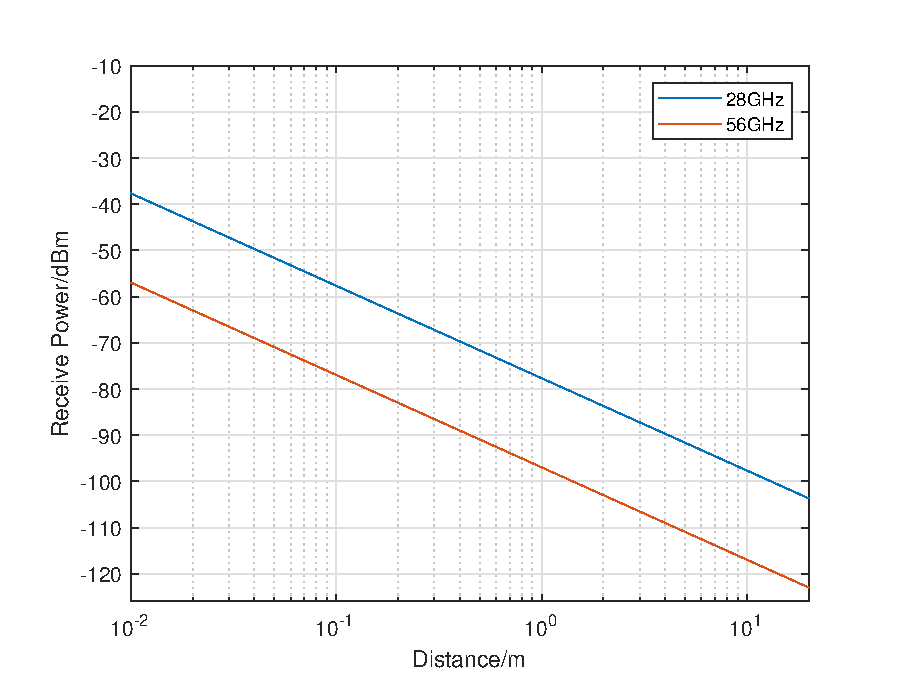
\includegraphics[width=0.6\textwidth]{Matlab/resPower.eps}
\caption{Received power over measurement distance at $P_{\text{TX}}=\SI{-13}{\decibelm}$}
\label{fig:resP}
\end{figure}

The \ac{LB} is the received power $P_{\text{RX}}$ with all losses and gains taken to account

\begin{equation}
P_{\text{RX}} = P_{\text{TX}}-L_{\text{TX}}+G_{\text{TX}}-L_{\text{FSPL}} + G_{\text{RX}}-L_{\text{RX}}\,.
\end{equation}

The global emission limit is (ref. section \ref{sec:legem} \cite{ceptercrec}, \cite{ansi}, \cite{fcc}) $\SI{-13}{\decibelm\per\mega\hertz}$. To evaluate sufficient measurement sensibility or measurement power budget the transmit power is set in fig. \ref{fig:resP} to $P_{\text{TX}}=\SI{-13}{\decibelm}$, the transmit cable loss is set to $L_{\text{TX}} = \SI{0}{\decibel}$, the most conservative assumption for the transmit antenna gain is $ G_{\text{TX}} = \SI{0}{\decibeli}$, the \ac{FSPL} is dependant on the distance $d$ so that 
\begin{equation}
L_{\text{FSPL}} = 20\log_{10}\left(4\pi d \cdot\lambda^{-1}\right)\si{\decibel}\,,
\label{eq:fspl}
\end{equation}
the receive antenna gain (Vivaldi antenna, compare fig. \ref{fig:ats}) is about $ G_{\text{RX}} = \SI{14}{\decibeli}$ and the receive cable loss is $L_{\text{RX}}=\SI{14}{\decibel}$. The resulting received power is depicted in fig. \ref{fig:resP}. This is valid for the ATS1000 antenna test system from \ac{RS}. Cable loss increases exponentially with the frequency and the length. Using a bigger chamber would cause longer cables and with that exponentially higher cable loss. This was not considered in fig. \ref{fig:resP}, which makes it best case. For the $\SI{56}{\giga\hertz}$ line the squared cable loss was assumed. In summary, for big chambers and high frequencies additional amplifiers are required.\\
The \ac{DANL} of the signal analyzers from \ac{RS} is depicted in annex \ref{fig:danl} with an \ac{RBW} of $f_{\text{RBW}}=\SI{1}{\hertz}$. At $\SI{28}{\giga\hertz}$ and with a \ac{RBW} of $f_{\text{RBW}}=\SI{1}{\mega\hertz}$ the noise level would be approximately $P_N \approx \SI{-100}{\decibelm}$. Regarding fig. \ref{fig:resP} for an ATS1000 with $d=\SI{0.5}{\meter}$ the dynamic range is about $\SI{30}{\decibel}$, whereas the dynamic range at $\SI{56}{\giga\hertz}$ would be less than $\SI{10}{\decibel}$. To increase the dynamic range an additional amplifier or a mixer at the probe antenna would be required.

\section{Quiet Zone / Measurement Uncertainties in ACs}

\begin{figure}[h]
  \centering
  \subfigure[Amplitude taper Vivladi TC-TA85CP]{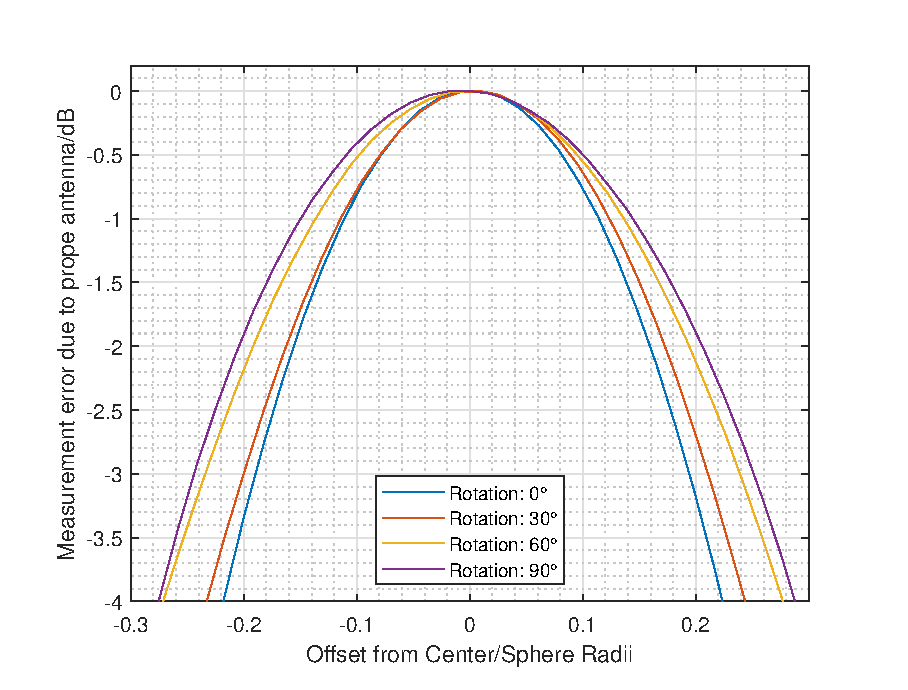
\includegraphics[width=0.49\textwidth]{Matlab/QZProbe.eps}}
  \centering
  \subfigure[Amplitude taper FSPL]{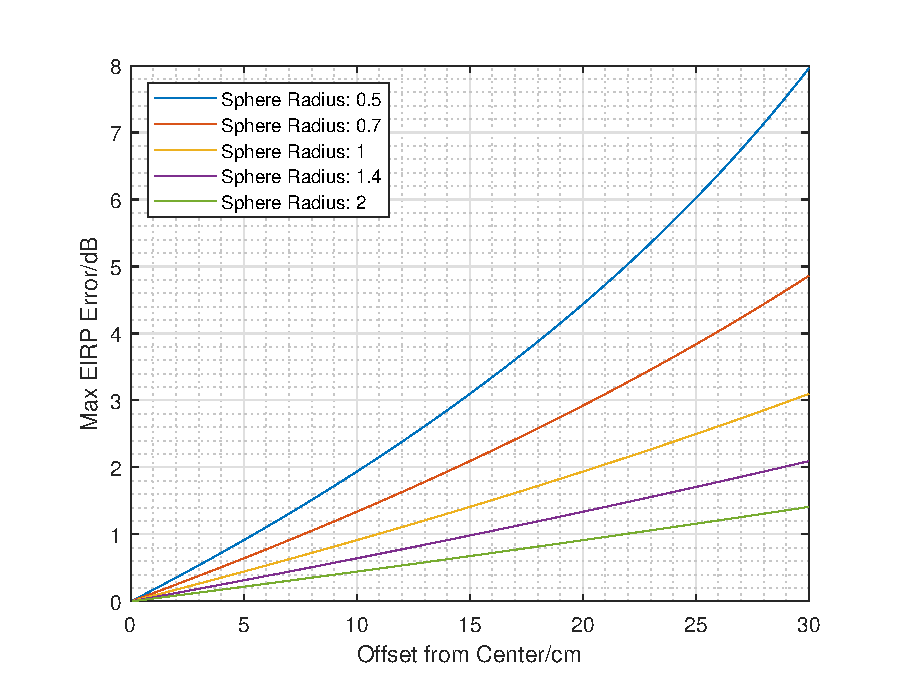
\includegraphics[width=0.49\textwidth]{Matlab/QZFSPL.eps}}
\caption{Quiet Zone sizes}
\label{fig:qz}
\end{figure}

Another criterion of an \ac{ATS} is the \ac{QZ}. The \ac{QZ} is a volume wherein correct \ac{OTA} measurements can be carried out, the wave fronts are plane and $E$ and $H$ fields are coherent with a known maximum taper. It's size is dependent from the absorbers, the measurement distance and the probe antenna. Normally a amplitude taper of around $\SI{1}{\decibel}$ is accepted.\\
The probe antenna should have a constant sensitivity at the \ac{QZ}. To illustrate that the pattern of the \ac{RS} TC-TA85CP Vivaldi antenna is plotted in fig. \ref{fig:qz} (a) expressed in sphere radii $r$. This is only valid for small angles with $a=r\cdot\sin \theta$. As an ATS1000 has a measurement distance of $d = \SI{0.5}{\meter}$, the \ac{QZ} would be around $\left(\SI{10}{\centi\meter}\right)^3$.\\
For a arbitrary radiating \ac{DUT} also the difference in \ac{FSPL} is a criterion for the \ac{QZ}-size. For that sake the error in \ac{FSPL} was computed by $\Delta P = 20\log_{10}\left(r\cdot\left(r-\Delta r\right)^{-1}\right)$ and depicted in fig. \ref{fig:qz} (b). The \ac{QZ} is again about $\left(\SI{10}{\centi\meter}\right)^3$. The last criterion for the \ac{QZ} is that any reflection in the \ac{ATS} is lower then every relevant feature of the \ac{DUT}s radiation pattern.\cite{ach}\\
The \ac{QZ} size for \acp{CATR} is mainly dependent of the size of the used mirror, it's high frequency quality is correlated with the manufacturing quality of the mirror.

\section{VNA or VSA Detector Settings}

\begin{figure}[h]
\centering
\def\svgwidth{0.7\textwidth}
\input{Bilder/detectorSetting.pdf_tex}
\caption{Comparison of Detector Settings \cite{funsspec}}
\label{fig:detset}
\end{figure}

In this section the different \ac{VNA} or \ac{VSA} detector settings are introduced. With the detector a certain sample in a given interval is chosen, compare fig. \ref{fig:detset}. There are six main settings for the detector: \cite{funsspec}
\begin{itemize}
\item The \textcolor[RGB]{237,28,36}{Max Peak-detector} takes the maximum value in the given interval.
\item The \textcolor[RGB]{0,166,88}{Min Peak-detector} takes the minimum value in the given interval.
\item The \textcolor[RGB]{0,94,138}{Auto Peak-detector} displays the interval from Min- to Max-Peak.
\item The \textcolor[RGB]{0,173,239}{Sample-detector} takes the first value in the given interval.
\item The \textcolor[RGB]{246,135,18}{RMS-detector} computes the \ac{RMS} of the signal to display.
\item The \textcolor[RGB]{114,100,184}{AV-detector} computes the average of the signal to display.
\end{itemize}

\begin{figure}
\centering
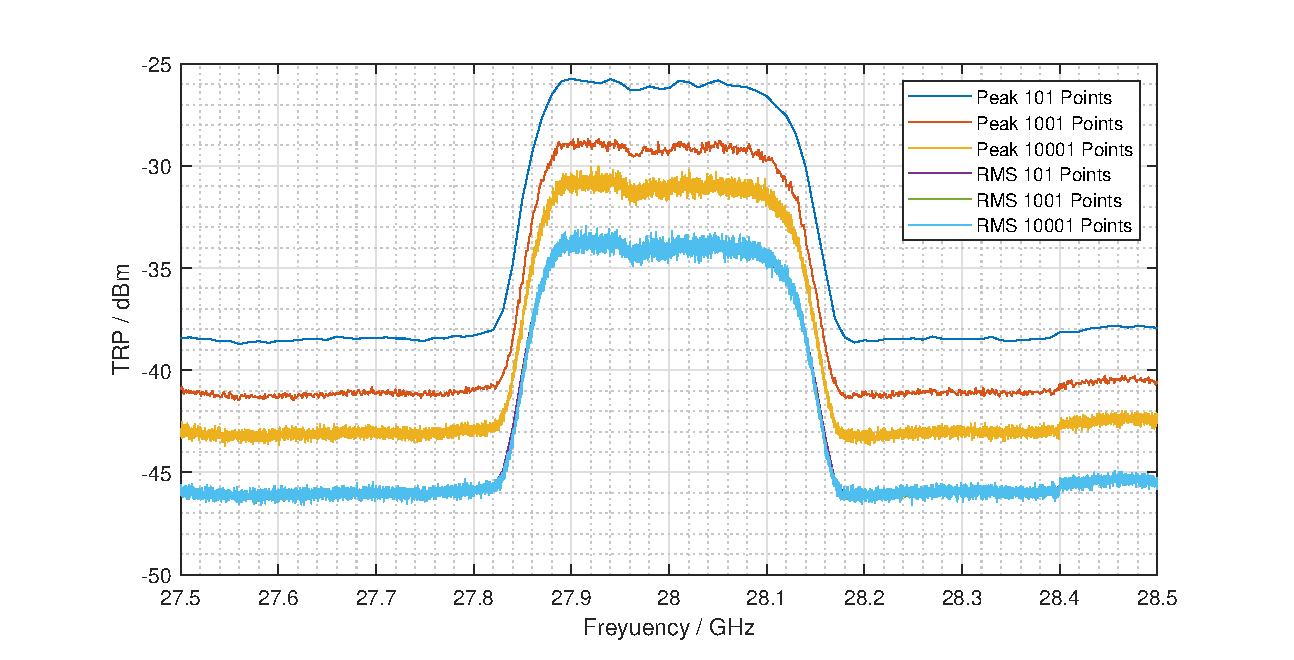
\includegraphics[width=0.8\textwidth]{Matlab/CompareDet.eps}
\caption{TRP measurement of noise with different detector settings}
\label{fig:trpmeasnoise}
\end{figure}

Choosing the correct detector setting is dependent of the expected signal. If a stochastic signal (noise) is to be found, the \ac{RMS}-detector is always the best choice. If it is harmonic, the Max Peak-detector is best. This phenomenon is depicted in fig. \ref{fig:trpmeasnoise}, where a \ac{TRP} measurement of a wideband white noise was accomplished. This measurement was done with a \ac{RBW} of $\SI{1}{\mega\hertz}$ and a sweep time of $\SI{4}{\milli\second}$. With \ac{RMS} detector the outcome is independent from the number of points, while the peak detectors is, because of the greater possibility for a great values in broader intervals, dependent of the number of points. This leads to two major issues:

\begin{enumerate}
\item By using the Peak-detector for measuring stochastic signals the minimum error is $\SI{2.5}{\decibel}$ when the frequency intervals are short (a lot of display points).
\item If the \ac{RMS}- or AV-detector is used harmonic signals are underrated dependent from the interval length caused by the averaging.
\end{enumerate} 

It is common practise for \ac{SE} measurements to perform a coarse pre scan with Peak-detector followed by a fine scan with \ac{RMS} detector at the spots in the spectra where emissions close to the limit are found.


